\section{Spending Functions \label{sec:spendfn}}

\subsection{Spending function definitions.} For any given $0<\alpha<1$ we define a non-decreasing function $f(t; \alpha)$ for $t\geq 0$ with $\alpha\left(  0\right)  =0$ and for $t\geq 1$, 
$f( t; \alpha)  =\alpha$. 
For $i=1,2,\ldots,K$ we define $t_i=I_{i}/I_{K}$ and then set $\alpha_i(0)$ through the equation
\begin{equation}
f(t_i;\alpha)=\sum_{j=1}^{i}\alpha_{j}(0).\label{alpha spending}%
\end{equation}
We consider a spending function proposed by Lan and DeMets \cite{LanDeMets} to approximate a Pocock bound. 
\begin{equation}
f(t; \alpha)=\alpha\log(1+(e-1)t)\label{eq:sfLDPocock}
\end{equation}
This spending function is implemented in the function \texttt{sfLDPocock}.
We again consider a 2-sided design with equally spaced analyses, $t_i=i/4$, $i=1,2,3,4$.
The values for $\alpha_i(0)$ are obtained as follows:
\begin{verbatim}
> sfLDPocock(alpha=.025, t=1:4/4)$spend
[1] 0.00893435 0.01550286 0.02069972 0.02500000
\end{verbatim}
We will discuss the exact nature of this call to \texttt{sfLDPocock} in Section \ref{sec:sfDetails} below.
We now derive a design for the CAPTURE study using this spending function
\begin{verbatim}
> n.fix <- nBinomial(p1=.15, p2=.1, beta=.2)
> x <- gsDesign(k=4, test.type=2, n.fix=n.fix, sfu=sfLDPocock, beta=.2)
> cumsum(x$upper$prob[,1])
[1] 0.00893435 0.01550287 0.02069973 0.02500001
\end{verbatim}
The boundary crossing probabilities under the assumption of no treatment difference are in \texttt{x\$upper\$prob[,1]} and there cumulative totals are produced by the above call to \texttt{cumsum()}. 
Note that these values match those produced by the call to \texttt{sfLDPocock} above.
Next we compare the bounds produced by this design with the actual Pocock bounds to see they are nearly identical:
\bigskip
\begin{verbatim}
> xPocock <- gsDesign(k=4, test.type=2, n.fix=n.fix, sfu="Pocock", beta=.2)
> x$upper$bound
[1] 2.368328 2.367524 2.358168 2.350030
> xPocock$upper$bound
[1] 2.361298 2.361298 2.361298 2.361298
>
\end{verbatim}
\bigskip

The reader may wish to compare the O'Brien-Fleming design presented in \ref{sec:boundfam} using the spending function \texttt{sfLDOF}, which implements a spending function proposed by Lan and DeMets \cite{LanDeMets} to approximate this design:
\begin{equation}
\alpha_i(t)=2\left(  1-\Phi\left(  \frac{\Phi
^{-1}(\alpha/2)}{\sqrt{t}}\right)  \right)
\end{equation}
You will see that this approximation is not as good as the Pocock bound approximation.
\subsection{Spending function families}
The function $f(t;\alpha)$ may be generalized to a family $f(t;\alpha,\gamma)$ of spending functions using one or more parameters. 
For instance, the default Hwang-Shih-DeCani spending function family is defined for $0\leq t\leq 1$ and any real $\gamma$ by
\[
f(t;\alpha, \gamma)=%
\begin{array}
[c]{cc}%
\alpha\frac{1-\exp(-\gamma t)}{1-\exp(-\gamma)}, & \gamma\neq 0\\
\alpha t, & \gamma=0
\end{array}
\]

The boundary crossing probabilities $\alpha_i^{+}(\theta)$ and $\beta_i(\theta)$ may be defined in a similar fashion, $i=1,2,\ldots,K$ with the same or different spending functions $f$ where: 
\begin{eqnarray}
f(t_i;\alpha)&=&\sum_{j=1}^{i}\alpha_{j}^{+}(0)\label{alpha+spending}\\
f(t_i;\beta(\theta))&=&\sum_{j=1}^{i}\beta_j(\theta)\label{betaspending}
\end{eqnarray}

The argument \texttt{test.type} in \texttt{gsDesign()} provides two options for how to use (\ref{betaspending}) to set lower bounds. 
For \texttt{test.type}=2, 5 and 6, lower boundary values are set under
the null hypothesis by specifying $\beta(t;0),$ $0\leq t$. 
For \texttt{test.type}=3 and 4, we compute lower boundary values under the
alternative hypothesis by specifying $\beta(t;\delta)$, $0\leq t$.
$\beta(t;\delta)$ is referred to as the $\beta$-spending function and the
value $\beta_{i}(\delta)$ is referred to as the amount of $\beta$ (Type
II error rate) spent at analysis $i$, $1\leq i\leq K$.

Standard published spending functions commonly used for group sequential
design are included as part of the gsDesign package. 
Several `new' spending functions are included that are of potential interest. 
Users can also write their own spending functions to pass directly to \texttt{gsDesign()}. 
Available spending functions and the syntax for writing a new spending function are documented here. 
We begin here with simple examples of how to apply standard spending functions in calls to \texttt{gsDesign()}. 
This may be as far as many readers may want to read. 
However, for those interested in more esoteric spending functions, full documentation of the extensive spending function capabilities available is included. 
Examples for each type of spending function in the package are included in the online help documentation.

\subsection{Spending Function Basics}

The parameters \texttt{sfu} and \texttt{sfl} are used to set spending functions for the upper and lower bounds, respectively, each having a default value of \texttt{sfHSD}, the Hwang-Shih-DeCani spending function.
The default parameter for the upper bound is $\gamma = -4$ to produce a conservative, O'Brien-Fleming-like bound. 
The default for the lower bound is $\gamma = -2$, a less conservative bound. 
This design was presented at some length in \ref{sec:default}.

To change these to $-3$ (less conservative than an O'Brien-Fleming bound) and $1$ (an aggressive Pocock-like bound), respectively, requires the parameter \texttt{sfupar} for the upper bound and \texttt{sflpar} for the lower bound:
Next we consider some simple alternatives to the default spending function parameters.
The Kim-DeMets function, \texttt{sfPower()}, with upper bound parameter $\rho
= 3$ (a conservative, O'Brien-Fleming-like bound) and lower bound parameter
$\rho = 0.75$ (an aggressive, Pocock-like bound) requires resetting the upper bound spending function \texttt{sfu} and the lower bound spending function \texttt{sfl}.
In the first code line following, we replace lower and upper spending function parameters with $1$ and $-2$, respectively; the default Hwang-Shih-DeCani spending function family is still used. 
In the second line, we specify a Kim-DeMets (power) spending function for
both the lower bound (with the parameters \texttt{sfl=sfPower} and \texttt{sflpar=2}) and the upper bounds (with the parameters \texttt{sfu=sfPower} and \texttt{sfupar=3}).
Then we compare bounds from the three designs. 
Bounds for the power spending function design are quite comparable to the default design. Generally, choosing between these two spending function families is somewhat arbitrary. The alternate Hwang-Shih-DeCani design uses more aggressive stopping boundaries. The last lines below show that sample size inflation from a fixed design is about 25\% for the the design with more aggressive stopping boundaries compared to about 7\% for each of the other designs. 

\bigskip

\begin{verbatim}
> x <- gsDesign()
> xHSDalt <- gsDesign(sflpar=1, sfupar=-2)
> xKD <- gsDesign(sfl=sfPower, sflpar=2, sfu=sfPower, sfupar=3)
> x$upper$bound
[1] 3.010739 2.546531 1.999226
> xHSDalt$upper$bound
[1] 2.677524 2.385418 2.063740
> xKD$upper$bound
[1] 3.113017 2.461933 2.008705
> x$lower$bound
[1] -0.2387240  0.9410673  1.9992264
> xHSDalt$lower$bound
[1] 0.3989132 1.3302944 2.0637399
> xKD$lower$bound
[1] -0.3497491  0.9822541  2.0087052
> x$n.I[3]
[1] 1.069883
> xHSDalt$n.I[3]
[1] 1.254268
> xKD$n.I[3]
[1] 1.071011
>\end{verbatim}

Following is example code to plot Hwang-Shih-DeCani spending
functions for three values of the $\gamma$ parameter. The first two $\gamma$
values are the defaults for upper bound spending ($\gamma = -4$; a conservative
bound somewhat similar to an O'Brien-Fleming bound) and lower bound spending
($\gamma = -2$; a less conservative bound). The third ($\gamma = 1$) is
included as it approximates a Pocock stopping rule; see Hwang, Shih and DeCani
\cite{HwangShihDeCani}. The Hwang-Shih-DeCani spending function class
implemented in the function \texttt{sfHSD()} may be sufficient for designing
many clinical trials without considering the other spending function forms
available in this package. The three parameters in the calls to 
\texttt{sfHSD()}%
\ below are the total Type I\ error, values for which the spending function is
evaluated (and later plotted), and the $\gamma$ parameter for the
Hwang-Shih-DeCani design. 
The code
below yields the plot in Figure~\ref{fig:hsd} below (note the typesetting of Greek characters!):

\bigskip

\begin{verbatim}
> plot(0:100/100, sfHSD(.025, 0:100/100, -4)$spend, type="l", lwd=2,
+      xlab="Proportion of information",
+      ylab=expression(paste("Cumulative \ ",alpha,"-spending")),
+      main="Hwang-Shih-DeCani Spending Functions")
> lines(0:100/100, sfHSD(.025, 0:100/100, -2)$spend, lty=2, lwd=2)
> lines(0:100/100, sfHSD(.025, 0:100/100, 1)$spend, lty=3, lwd=2)
> legend(x=c(.0, .27), y=.025 * c(.8, 1), lty=1:3, lwd=2,
+        legend=c(expression(paste(gamma," = -4")),
+                 expression(paste(gamma," = -2")),
+                 expression(paste(gamma," = 1"))))
\end{verbatim}
\bigskip

Similarly, Jennison and Turnbull \cite{JTBook},
suggest that the Kim-DeMets spending function is flexible enough to suit most
purposes. To compare the Kim-DeMets family with the Hwang-Shih-DeCani family
just demonstrated, substitute \texttt{sfPower()} instead of
\texttt{sfHSD()}; use parameter values $3$, $2$ and $0.75$ to 
replace the values $-4$,$-2$, and $1$ in the code shown above: 

\bigskip
\begin{verbatim}
> plot(0:100/100,sfPower(.025, 0:100/100, 3)$spend, type="l", lwd=2,
+      xlab="Proportion of information",
+      ylab=expression(paste("Cumulative \ ",alpha,"-spending")),
+      main="Kim-DeMets Spending Functions")
> lines(0:100/100, sfPower(.025, 0:100/100, 2)$spend, lty=2, lwd=2)
> lines(0:100/100, sfPower(.025, 0:100/100, 0.75)$spend, lty=3, lwd=2)
> legend(x=c(.0, .27), y=.025 * c(.8, 1), lty=1:3, lwd=2,
+        legend=c(expression(paste(gamma," = 3")),
+                 expression(paste(gamma," = 2")),
+                 expression(paste(gamma," = 0.75"))))
\end{verbatim}

\bigskip 

\begin{center}%
\begin{figure}
\begin{center}
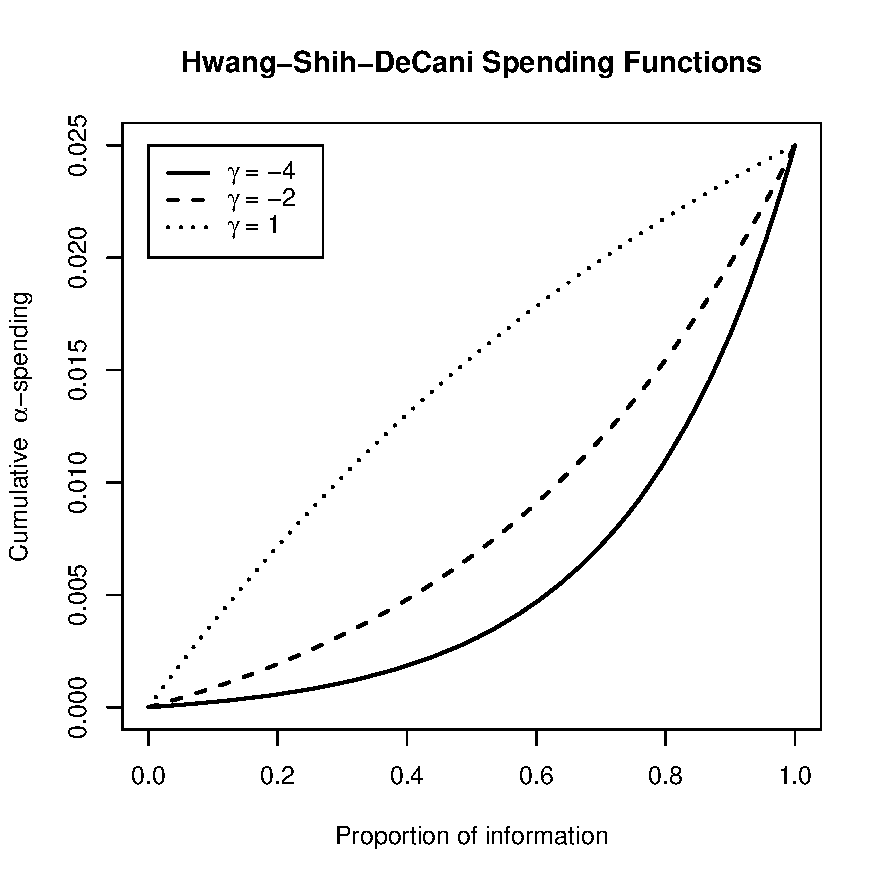
\includegraphics[width=.6\textwidth]{figs/HSDexample.pdf}
\end{center}
\caption{Hwang-Shih-DeCani spending function example\label{fig:hsd}}
\end{figure}%

\end{center}

\subsection{Resetting timing of analyses\label{sec:reset}}

When designed with a spending function, the timing and number of analyses may
be altered during the course of the trial. \ This is very easily handled in
the \texttt{gsDesign()} routine using the input arguments \texttt{n.I} and
\texttt{maxn.IPlan}. We demonstrate this by example. Suppose a trial was
originally designed with the call:

\bigskip

\begin{verbatim}
> x <- gsDesign(k=5, n.fix=800)
> x$upper$bound
> x$n.I
\end{verbatim}

\bigskip

The second and third lines above show the planned upper bounds and sample
sizes at analyses. Suppose that when executed the final interim was skipped,
the first 2 interims were completed on time, the third interim was completed
at 575 patients (instead of 529 as originally planned), the fourth interim was
skipped, and the final analysis was performed after 875 patients (instead of
after 882 as originally planned). The boundaries for the analyses can be
obtained as follows:

\bigskip
\begin{verbatim}
> gsDesign(k=4, n.fix=800, n.I=c(177,353,575,875), maxn.IPlan=x$n.I[x$k])
\end{verbatim}

\bigskip

This design now has slightly higher power (90.4\%) than the originally planned
90\%. This is because the final boundary was lowered relative to the original
plan when the $\alpha$-spending planned for the fourth interim was saved
for the final analysis by skipping the final interim. Note that all of the
arguments for the original design must be supplied when the study is
re-designed---in addition to adding \texttt{n.I}, which may have the same
number, fewer, or more interim analyses compared to the original plan. If the
sample size for the final analysis is changed, \texttt{maxn.IPlan} should be
passed in as the original final sample size in order to appropriately assign
$\alpha$- and $\beta$-spending for the interim analyses.


\section{Advanced spending function details\label{sec:sfDetails}}
\subsection{Spending functions as arguments\label{sec:sfArgs}}
Except for the "OF", "Pocock" and "WT" examples given in Section \ref{sec:boundfam}, a spending function passed to \texttt{gsDesign()} through the arguments \code{sfu} (upper bound) and \code{sfl} (lower bound) must have the following calling sequence:

\bigskip

\texttt{sfname(alpha, t, param)}

\bigskip

where \texttt{sfname} is an arbitrary name for a spending function available
from the package or written by the user. The arguments are as follows:

\begin{itemize}
\item \texttt{alpha}: a real value ($0 < \mathtt{alpha} < 1$).
The total error spending for the boundary to be determined. 
This would be replaced with the following values from a call to \texttt{gsDesign()}:
\texttt{alpha} for the upper bound, and either \texttt{beta} (for
\texttt{test.type = 3} or \texttt{4}) or \texttt{astar} (for 
\texttt{test.type = 5} or \texttt{6}) for the lower bound.

\item \texttt{t}: a vector of arbitrary length $m$ of real values, $0 \leq
t_{1} < t_{2} < \ldots t_{m}\leq1$. 
Specifies the proportion of spending for which values of the spending function are to be computed.

\item \texttt{param}: for all cases here, this is either a real value or a
vector of real values. One or more parameters that (with the parameter
\texttt{alpha}) fully specify the spending function. This is specified in
a call to \texttt{gsDesign()} with \texttt{sfupar} for the upper bound and
\texttt{sflpar} for the lower bound.
\end{itemize}

The value returned is of the class \texttt{spendfn} which was described in 
Section~\ref{sec:spendfn}, The \texttt{spendfn} Class.

The following code and output demomstrate that the default value \texttt{sfHSD} for the upper and lower spending functions \texttt{sfu} and \texttt{sfl} is a function:

\bigskip
\begin{verbatim}
> sfHSD
function (alpha, t, param) 
{
    checkScalar(param, "numeric", c(-40, 40))
    t[t > 1] <- 1
    x <- list(name = "Hwang-Shih-DeCani", param = param, parname = "gamma", 
        sf = sfHSD, spend = if (param == 0) t * alpha else alpha * 
            (1 - exp(-t * param))/(1 - exp(-param)), bound = NULL, 
        prob = NULL)
    class(x) <- "spendfn"
    x
}
<environment: namespace:gsDesign>
\end{verbatim}
\bigskip

Table 1 summarizes many spending functions available in the package. A basic
description of each type of spending function is given. The table begins with
standard spending functions followed by two investigational spending
functions: \texttt{sfExponential()} and \texttt{sfLogistic()}. These spending
functions are discussed further in Section~\ref{sec:invspendfun}, Investigational Spending Functions, but
are included here due to their simple forms. The logistic spending function
represented by \texttt{sfLogistic()} has been used in several trials. It
represents a class of two-parameter spending functions that can provide
flexibility not available from one-parameter families. The
\texttt{sfExponential()} spending function is included here as it provides an
excellent approximation of an O'Brien-Fleming design as follows:

\bigskip

\begin{verbatim}
gsDesign(test.type=2, sfu=sfExponential, sfupar=0.75)
\end{verbatim}
\bigskip

See also subsections below and online documentation of spending functions.

\bigskip

\begin{table}
\caption{Spending function definitions and parameterizations.}
\begin{tabular}
[c]{cccc}\hline
Function & Spending Function & Functional & Parameter\\
(parameter) & Family & Form & (\texttt{sfupar} or \texttt{sflpar})\\\hline
\texttt{sfHSD} & Hwang-Shih- &  & Value in [-40,40).\\
\texttt{\ (gamma)} & DeCani & $\alpha\frac{1-\exp(-\gamma t)}{1-\exp(-\gamma
)}$ & -4=O'Brien-Fleming like;\\
&  &  & 1=Pocock-like\\\hline
\texttt{sfPower} &  &  & Value in $(0,+\infty)$\\
\texttt{(rho)} & Kim-DeMets & $\alpha t^{\rho}$ & 3=O'Brien-Fleming like\\
&  &  & 1=Pocock-like\\\hline
\texttt{sfLDPocock} & Pocock & $\alpha\log(1+(e-1)t)$ & None\\
\texttt{(none)} & approximation &  & \\\hline
\texttt{sfLDOF } & O'Brien-Fleming & $2\left(  1-\Phi\left(  \frac{\Phi
^{-1}(\alpha/2)}{\sqrt{t}}\right)  \right)  $ & None\\
\texttt{(none)} & approximation &  & \\\hline
\texttt{sfLinear} & Piecewise linear & Specified points & Cumulative proportion of\\
\texttt{(t}$_{1}$,\texttt{t}$_{2}$,...,\texttt{t}$_{m}$\texttt{)}
&specification 
& $0<t_{1}\ldots<t_{m}<1$ 
& information and error\\
\texttt{(p}$_{1}$,\texttt{p}$_{2}$,...,\texttt{p}$_{m}$\texttt{)} 
&& $0<p_{1}\ldots<p_{m}<1$
& spending for given timepoints\\\hline
\texttt{sfExponential} &  &  & $(0,10]$\\
\texttt{(nu)} & Exponential & $\alpha^{t^{-\nu}}$ & Recommend $\nu<1$\\
&  &  & $0.75=$O'Brien-Fleming-like\\\hline
\texttt{sfLogistic} & Logistic & $\alpha\frac{e^{a}\left(  \frac{t}
{1-t}\right)  ^{b}}{1+e^{a}\left(  \frac{t}{1-t}\right)  ^{b}}$ & $b>0$\\
\texttt{(a,b)} &  &  & \\\hline
\texttt{"WT"} & Wang-Tsiatis & $C(k,\alpha,\Delta)(i/K)^{\Delta-1/2}$ &
0=O'Brien-Fleming bound\\
\texttt{(Delta)} & bounds &  & 0.5=Pocock bound\\\hline
\texttt{"Pocock"} & Pocock &  & This is a special case\\
\texttt{(none)} & bounds &  & of WT with $\Delta=1/2.$\\\hline
\texttt{"OF"} & O'Brien-Fleming &  & This is a special case\\
\texttt{(none)} & bounds &  & of WT with $\Delta=0.$\\\hline
\end{tabular}
\end{table}

\subsection{Investigational spending functions\label{sec:invspendfun}}

When designing a clinical trial with interim analyses, the rules for stopping
the trial at an interim analysis for a positive or a negative efficacy result
must fit the medical, ethical, regulatory and statistical situation that is
presented. Once a general strategy has been chosen, it is not unreasonable to
discuss precise boundaries at each interim analysis that would be considered
ethical for the purpose of continuing or stopping a trial. Given such
specified boundaries, we discuss here the possibility of numerically fitting
$\alpha$- and $\beta$-spending functions that produce these boundaries.
Commonly-used one-parameter families may not provide an adequate fit to
multiple desired critical values. We present a method of deriving
two-parameter families to provide some additional flexibility along with
examples to demonstrate their usefulness. This method has been found to be
useful in designing multiple trials, including the CAPTURE\ trial
\cite{CAPTURE}, the GUSTO\ V trial \cite{GUSTOV} and three ongoing trials at Merck.

One method of deriving a two-parameter spending function is to use the
incomplete beta distribution which is commonly denoted by $I_{x}(a,b)$ where
$a>0$, $b>0$. We let%
\[
\alpha(t;a,b)=\alpha I_{t}(a,b).
\]
This spending function is implemented in \texttt{sfBetaDist()}; developing
code for this is also demonstrated below in Section~\ref{sec:newspendfn},
Writing Code for a New Spending Function.

Another approach allows fitting spending functions by solving a linear system
of 2 equations in 2 unknowns. A two-parameter family of spending function is
defined using an arbitrary, continuously increasing cumulative distribution
function $F()$ defined on $(-\infty, \infty)$, a real-valued parameter $a$ and
a positive parameter $b$:
\begin{equation}
\alpha(t;a,b)=\alpha F(a+bF^{-1}(t)).\label{2 param sf}%
\end{equation}
Fix two points of the spending function 
$0 < \mathtt{t0} < \mathtt{t1} < 1 $ to have spending function values specified by \texttt{u0} $\times
$ \texttt{alpha} and \texttt{u1} $\times$ \texttt{alpha}, respectively, where 
$0 < \mathtt{u0} < \mathtt{u1} < 1$. Equation (\ref{2 param sf}) now yields two linear equations with two
unknowns, namely for $i=1,2$
\[
F^{-1}(u_{i})=a+bF^{-1}(t_{i}).
\]
The four value specification of \texttt{param} for this family of spending
functions is \texttt{param=c(t0, t1, u0, u1)} where the objective is that
\texttt{sf(t0) = alpha*u0} and \texttt{sf(t1) = alpha*u1}. In this
parameterization, all four values must be between 0 and 1 and 
$\mathtt{t0} < \mathtt{t1}$, $\mathtt{u0} < \mathtt{u1}$.

The logistic distribution has been used with this strategy to
produce spending functions for ongoing trials at Merck Research Laboratories
in addition to the GUSTO V trial \cite{GUSTOV}. The logit function is defined
for $0<u<1$ as ${\rm logit}(u)=\log(u/(1-u))$. Its inverse is defined for
$x\in(-\infty,\infty)$ as ${\rm logit}^{-1}(x)=e^{x}/(1+e^{x})$. Letting $b>0$,
$c=e^{a}>0$, $F(x)={\rm logit}^{-1}(x)$ and applying (\ref{2 param sf}) we obtain
the logistic spending function family:
\begin{align}
\alpha(t;a,b)  & =\alpha\times {\rm logit}^{-1}(\log(c)+b\times
{\rm logit}(u))\label{logistic sf}\\
& =\alpha\frac{c\left(  \frac{t}{1-t}\right)  ^{b}}{1+c\left(  \frac{t}%
{1-t}\right)  ^{b}}%
\end{align}
The logistic spending function is implemented in \texttt{sfLogistic()}.
Functions are also available replacing $F()$ with the cumulative distribution
functions for the standard normal distribution (\texttt{sfNormal()}), two
versions of the extreme value distribution (sfExtremeValue() with
$F(x)=exp(-exp(-x)$) and sfExtremeValue2 with $F(x)=1-exp(-exp(x))$), the
central t-distribution (\texttt{sfTDist()}), and the Cauchy distribution
(\texttt{sfCauchy()}). Of these, \texttt{sfNormal()} is fairly similar to
\texttt{sfLogistic()}. \ On the other hand, \texttt{sfCauchy()} can behave
quite differently. The function \texttt{sfTDist()} provides intermediary
spending functions bounded by \texttt{sfNormal()} and \texttt{sfCauchy()}; it
requires an additional parameter, the degrees of freedom \ See online help for
more complete documentation, particularly for \texttt{sfTDist()}. \ Following
is an example that plots several of these spending functions that fit through
the same two points (\texttt{t1}=0.25, \ \texttt{t2}=0.5, \texttt{u1}=0.1,
\texttt{u2}=0.2) but behave differently for $t>1/2$.

\bigskip

\begin{verbatim}
> plotsf <- function(alpha,t,param)
{
    plot(t, sfCauchy(alpha, t, param)$spend, lwd=2,
         xlab="Proportion of enrollment",
         ylab="Cumulative spending", type="l")
    lines(t, sfLogistic(alpha, t, param)$spend, lty=4, lwd=2)
    lines(t, sfNormal(alpha, t, param)$spend, lty=5, lwd=2)
    lines(t, sfTDist(alpha, t, c(param, 1.5))$spend, lty=2, lwd=2)
    lines(t, sfTDist(alpha, t, c(param,2.5))$spend, lty=3, lwd=2)
    legend(x=c(.0, .3), y=alpha * c(.7,1), lty=1:5, lwd=2,
           legend=c("Cauchy", "t 1.5 df", "t 2.5 df", "Logistic", "Normal"))
}
> t <- 1:199/200
> t <- c(t, .9975, .99875, .9995, .99975)
> param <- c(.25, .5, .1, .2)
> plotsf(.025,t,param)
\end{verbatim}

\begin{center}%
\begin{figure}
\begin{center}
\includegraphics[width=.6\textwidth]{figs/sfLogistic.pdf}
\end{center}
\caption{Example fitting two- and three-parameter spending functions}
\end{figure}%

\end{center}

\subsection{Optimized spending functions}

The following two examples demonstrate some of the flexibility and research
possibilities for the \texttt{gsDesign} package. The particular examples may or may not
be of interest, but the strategy may be applied using a variety of
optimization criteria. First, we consider finding a spending function to match
a Wang-Tsiatis design. This could be useful to adjust a Wang-Tsiatis design if
the timing of interim analyses are not as originally planned. Second, we
replicate a result from Anderson \cite{AndBMJ} which minimized expected value
of the square of sample size over a family of spending functions and a prior distribution.

\begin{example}
Approximating a Wang-Tsiatis design
\end{example}

We have noted several approximations of O'Brien-Fleming and Pocock spending
rules using spending functions in the table above. Following is sample code to
provide a good approximation of Wang-Tsiatis bounds with a given parameter
$\Delta$. \ This includes O'Brien-Fleming ($\Delta$=0) and Pocock ($\Delta
$=0.5) designs. First, we define a function that computes the sum of squared
deviations of the boundaries of a Wang-Tsiatis design compared to a
one-parameter spending function family with a given parameter value of
\texttt{x}. Note that \texttt{Delta} is the parameter for the Wang-Tsiatis
design that we are trying to approximate. Other parameters are as before;
recall that \texttt{test.type} should be limited to 1 or 2 for Wang-Tsiatis
designs. Defaults are used for parameters for \texttt{gsDesign()} not included here.

\bigskip

\begin{verbatim}
WTapprox <- function(x, alpha=0.025, beta=.1, k=3, sf=sfHSD, 
                     Delta=.25, test.type=2)
{
    # Wang-Tsiatis comparison with a one-parameter spending function
    y1 <- gsDesign(k=k, alpha=alpha, beta=beta, test.type=test.type, sfu="WT",
                   sfupar=Delta)$upper$bound
    y2 <- gsDesign(k=k, alpha=alpha, beta=beta, test.type=test.type, sfu=sf,
                   sfupar=x)$upper$bound
    z <- y1-y2
    return(sum(z*z))
}
\end{verbatim}
\bigskip

We consider approximating a two-sided O'Brien-Fleming design with \texttt{alpha}%
=0.025 (one-sided) using the exponential spending function. The function
\texttt{nlminb()} is a standard R function used for minimization. It minimizes
a function passed to it as a function of that function's first 
argument, which may be a vector. The first parameter of \texttt{nlminb()} is 
a starting value for the minimization routine. The second is the function to be
minimized. The parameter \texttt{lower} below provides a lower bound for first
argument to the function being passed to \texttt{nlminb()}. \ Following
parameters are fixed parameters for the function being passed to
\texttt{nlminb()}. The result suggests that for $k=4$, an exponential spending
function with $\nu=0.75$ approximates an O'Brien-Fleming design well.
Examining this same optimization for $k=2$ to 10 suggests that $\nu=0.75$
provides a good approximation of an O'Brien-Fleming design across this range.

\bigskip

\begin{verbatim}
> nu <- nlminb(.67, WTapprox, lower=0, sf=sfExponential, k=4, Delta=0, test.type=2)$par
> nu
[1] 0.7562779
\end{verbatim}
\bigskip

Running comparable code for \texttt{sfHSD()} and \texttt{sfPower()}
illustrates that the exponential spending function can provide a better
approximation of an O'Brien-Fleming design than either the Hwang-Shih-DeCani
or Kim-DeMets spending functions. For Pocock designs, the Hwang-Shih-DeCani
spending function family provides good approximations.

\begin{example}
\bigskip Minimizing the expected value of a power of sample size
\end{example}

In this example, we first define a function that computes a weighted average
across a set of \texttt{theta} values of the expected value of a given power
of the sample size for a design. \ Note that \texttt{sfupar} and
\texttt{sflpar} are specified in the first input argument so that they may later
be optimized using the R routine \texttt{nlminb()}. The code is compact, which
is very nice for writing, but it may be difficult to interpret. A good way to
see how the code works is to define values for all of the parameters and run
each line from the R command prompt, examining the result.

\bigskip

\begin{verbatim}
# Expected value of the power of sample size of a trial 
# as a function of upper and lower spending parameter. 
# Get sfupar from x[1] and sflpar from x[2].
# val is the power of the sample size for which expected
#    values are computed.
# theta is a vector for which expected values are to be computed.
# thetawgt is a vector of the same length used to compute a
#    weighted average of the expected values.
# Other parameters are as for gsDesign.

enasfpar <- function(x, timing=1, theta, thetawgt, k=4, 
                     test.type=4, alpha=0.025, beta=0.1, 
                     astar=0, delta=0, n.fix=1, sfu=sfHSD, 
                     sfl=sfHSD, val=1, tol=0.000001, r=18)
{
    # derive design
    y <- gsDesign(k=k, test.type=test.type, alpha=alpha, beta=beta,
                  astar=astar, delta=delta, n.fix=n.fix, timing=timing,
                  sfu=sfu, sfupar=x[1], sfl=sfl, sflpar=x[2], tol=tol, r=r)
    # compute boundary crossing probabilities for input theta
    y <- gsProbability(theta=theta, d=y)
    # compute sample sizes to the val power
    n <- y$n.I^val
    # compute expected values
    en <- n %*% (y$upper$prob + y$lower$prob)
    # compute weighted average of expected values
    en <- sum(as.vector(en) * as.vector(thetawgt))
    return(en)
}
\end{verbatim}
\bigskip

Now we use this function along with the R routine \texttt{nlminb()} which
finds a minimum across possible values of \texttt{sfupar} and \texttt{sflpar}.
The design derived using the code below and a more extensive discussion can be
found in \cite{AndBMJ}. The code above is more general than in \cite{AndBMJ},
however, as that paper was restricted to \texttt{test.type}=5 (the program
provided there also worked for \texttt{test.type}=6).

\bigskip

\begin{verbatim}
# example from Anderson (2006)
delta <- abs(qnorm(.025) + qnorm(.1))
# use normal distribution to get weights
x <- normalGrid(mu=delta, sigma=delta/2)
x <- nlminb(start=c(.7, -.8), enasfpar, theta=x$z, timing=1, 
       thetawgt=x$wgts, val=2, k=4, test.type=5, tol=0.0000001)
x$message
y <- gsDesign(k=4, test.type=5, sfupar=x$par[1], sflpar=x$par[2])
y
\end{verbatim}

\subsection{Writing code for a new spending function\label{sec:newspendfn}}

Following is sample code using a cumulative distribution function for a
beta-distribution as a spending function. Let B(a,b) denote the complete beta
function. The beta distribution spending function is denoted for any
fixed $a>0$ and $b>0$ by%
\[
\alpha(t)=\frac{\alpha}{B(a,b)}%
%TCIMACRO{\tint \limits_{0}^{t}}%
%BeginExpansion
{\textstyle\int\limits_{0}^{t}}
%EndExpansion
x^{a-1}(1-x)^{b-1}dx.
\]
This spending function provides much of the flexibility of spending functions
in the last subsection, but is not of the same general form. This sample code
is intended to provide guidance in writing code for a new spending function,
if needed.

\bigskip
\begin{verbatim}
# implementation of 2-parameter version of beta distribution spending function
# assumes t and alpha are appropriately specified (does not check!)
sfbdist <- function(alpha, t, param)
{
    # set up return list and its class
    x <- list(name="B-dist example", param=param, parname=c("a","b"), 
         sf=sfbdist, spend=NULL, bound=NULL, prob=NULL, errcode=0, 
         errmsg="No error")
    class(x) <- "spendfn"
    # check for errors in specification of a and b
    # gsReturnError is a simple function available from the 
    # package for saving errors in the returned value}
    if (length(param) != 2) 
    {
        return(gsReturnError(x,errcode=.3,
               errmsg="b-dist example spending function parameter must be of length 2"))
    }
    if (!is.numeric(param)) 
    {
        return(gsReturnError(x,errcode=.1,
               errmsg="Beta distribution spending function parameter must be numeric"))
    }
    if (param[1] <= 0) 
    {
        return(gsReturnError(x,errcode=.12,
               errmsg="1st Beta distribution spending function parameter must be > 0."))
    }
    if (param[2] <= 0) 
    {
        return(gsReturnError(x,errcode=.13,
               errmsg="2nd Beta distribution spending function parameter must be > 0."))
    }
    # set spending using cumulative beta distribution function and return
    x$spend <- alpha * pbeta(t, x$param[1], x$param[2])
    return(x)
}
\end{verbatim}
\bigskip

The flexibility of this spending function is demonstrated by the following
code which produces the plot below. Using a=$\rho$, b=1 produces a Kim-DeMets
spending function $\alpha t^{\rho}$ as shown by the solid line with $\rho$=2.
The dashed line (\texttt{a}=6, \texttt{b}=4) shows a spending function that is
conservative very early, but then aggressive in its spending pattern starting
after about 40\% of data are available. The dotted (\texttt{a}=0.5,
\texttt{b}=0.5) and dot-dashed (\texttt{a}=0.6, \texttt{b}=2) show
increasingly aggressive early spending. These may be useful in setting an
initial high futility bound when the first part of a trial is used as a proof
of concept for a clinical endpoint.

\bigskip

\begin{verbatim}
> # plot some beta distribution spending functions
> plot(0:100/100, sfbdist(1, 0:100/100, c(2,1))$spend, type="l", lwd=2,
+      xlab="Proportion of information",
+      ylab="Cumulative proportion of total spending",
+      main="Beta Distribution Spending Function Example")
> lines(0:100/100, sfbdist(1, 0:100/100, c(6,4))$spend, lty=2, lwd=2)
> lines(0:100/100, sfbdist(1, 0:100/100, c(.5,.5))$spend, lty=3, lwd=2)
> lines(0:100/100, sfbdist(1, 0:100/100, c(.6,2))$spend, lty=4, lwd=2)
> legend(x=c(.65, 1), y=1 * c(0, .25), lty=1:4, lwd=2,
+        legend=c("a=2, b=1", "a=6, b=4", "a=0.5,b=0.5", "a=0.6, b=2"))
\end{verbatim}
\begin{center}%
\begin{figure}
\begin{center}
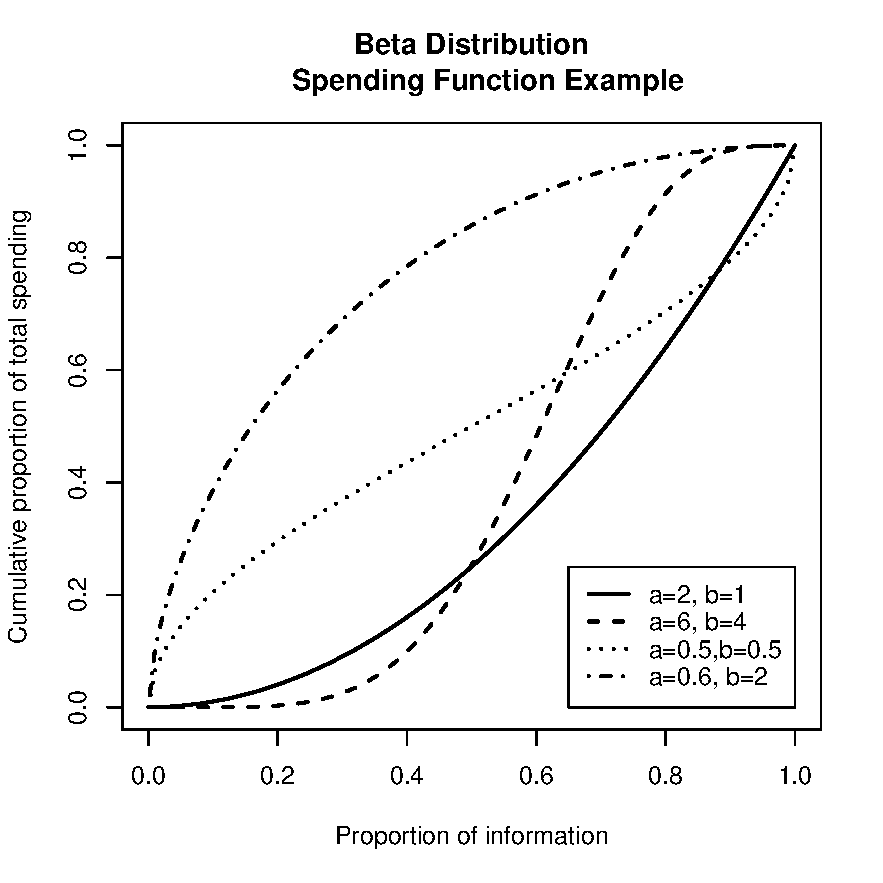
\includegraphics[width=.6\textwidth]{figs/sfbdist.pdf}
\end{center}
\caption{Example plotting user-written beta-distribution spending function}
\end{figure}%
%EndExpansion

\end{center}

